\section*{DNS}
The \texttt{nslookup} utility was used to do a DNS query on the \texttt{compeng4dn4.mooo.com} server. The terminal output of the DNS query is shown in Listing~\ref{list:dns_query}.

\begin{lstlisting}[caption=DNS Query Terminal Output,label=list:dns_query]
nslookup compeng4dn4.mooo.com
Server:  mynetwork
Address:  192.168.2.1

Non-authoritative answer:
Name:    compeng4dn4.mooo.com
Address:  99.236.34.223
\end{lstlisting}

The WireShark capture for the DNS query is shown below in Figure~\ref{fig:dns_query}. The capture was filtered for DNS queries containing \texttt{compeng4dn4.mooo.com}, using the display filter \texttt{dns.qry.name contains "compeng4dn4.mooo.com"}. 

The DNS query first searches for \texttt{compeng4dn4.mooo.com} with the DNS suffix \texttt{.home}, performing the query with "A" and "AAAA" records, for mapping hostnames to IPv4 and IPv6 addresses. Both DNS queries return "no such name" indicating that the queries are unsuccessful. The DNS query then queries \texttt{compeng4dn4.mooo.com} with no suffix, returning the correct IPv4 address for the A record. The AAAA record does not return any address.

\begin{figure}[htp]
\centering
\caption[dns_query]{DNS Query WireShark Capture}\label{fig:dns_query}
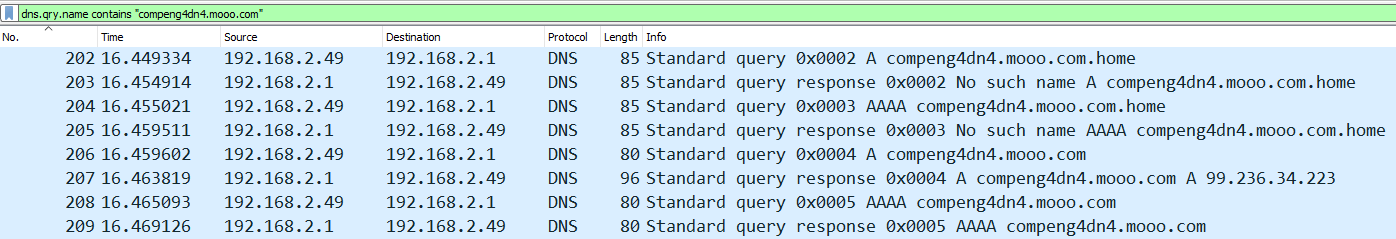
\includegraphics[width=\textwidth]{dns_query_wireshark.png}
\end{figure}